\documentclass[a4paper, 11pt, notitlepage, english]{article}

\usepackage{babel}
\usepackage[utf8]{inputenc}
\usepackage[T1]{fontenc, url}
\usepackage{textcomp}
\usepackage{amsmath, amssymb}
\usepackage{amsbsy, amsfonts}
\usepackage{graphicx, color, xcolor}
\usepackage{verbatim, listings, fancyvrb}
\usepackage{parskip}
\usepackage{framed}
\usepackage{amsmath}
\usepackage{multicol}
\usepackage{url}
\usepackage{flafter}
\usepackage{simplewick}
\usepackage{amsthm}
\usepackage{bbold}


\usepackage{caption}
\DeclareCaptionLabelSeparator{colon}{. }
\renewcommand{\captionfont}{\small\sffamily}
\renewcommand{\captionlabelfont}{\bf\sffamily}
\usepackage{float}
%\floatstyle{ruled}
%\restylefloat{figure}
\setlength{\captionmargin}{20pt}
%\addto\captionsenglish{\renewcommand{\figurename}{Fig.}}
\usepackage{bigstrut}
\setlength{\tabcolsep}{12pt}


\newtheorem{theorem}[]{Wick's Theorem}[]

\DeclareUnicodeCharacter{00A0}{~}

\definecolor{javared}{rgb}{0.6,0,0} % for strings
\definecolor{javagreen}{rgb}{0.25,0.5,0.35} % comments
\definecolor{javapurple}{rgb}{0.5,0,0.35} % keywords
\definecolor{javadocblue}{rgb}{0.25,0.35,0.75} % javadoc

\lstset{language=python,
basicstyle=\ttfamily\scriptsize,
keywordstyle=\color{javapurple},%\bfseries,
stringstyle=\color{javared},
commentstyle=\color{javagreen},
morecomment=[s][\color{javadocblue}]{/**}{*/},
morekeywords={super, with},
% numbers=left,
% numberstyle=\tiny\color{black},
stepnumber=2,
numbersep=10pt,
tabsize=2,
showspaces=false,
captionpos=b,
showstringspaces=false,
frame= single,
breaklines=true}

\usepackage{geometry}
\geometry{headheight=0.01mm}
\geometry{top=20mm, bottom=20mm, left=34mm, right=34mm}

\renewcommand{\arraystretch}{2}
\setlength{\tabcolsep}{10pt}
\makeatletter
\renewcommand*\env@matrix[1][*\c@MaxMatrixCols c]{%
  \hskip -\arraycolsep
  \let\@ifnextchar\new@ifnextchar
  \array{#1}}
%
% Definering av egne kommandoer og miljøer
%
\newcommand{\dd}[1]{\ \text{d}#1}
\newcommand{\f}[2]{\frac{#1}{#2}} 
\newcommand{\beq}{\begin{equation}}
\newcommand{\eeq}{\end{equation}}
\newcommand{\bra}[1]{\langle #1|}
\newcommand{\ket}[1]{|#1 \rangle}
\newcommand{\braket}[2]{\langle #1 | #2 \rangle}
\newcommand{\brakket}[2]{\langle #1 || #2 \rangle}
\newcommand{\braup}[1]{\langle #1 \left|\uparrow\rangle\right.}
\newcommand{\bradown}[1]{\langle #1 \left|\downarrow\rangle\right.}
\newcommand{\av}[1]{\left| #1 \right|}
\newcommand{\op}[1]{\hat{#1}}
\newcommand{\braopket}[3]{\langle #1 | {#2} | #3 \rangle}
\newcommand{\ketbra}[2]{\ket{#1}\bra{#2}}
\newcommand{\pp}[1]{\frac{\partial}{\partial #1}}
\newcommand{\ppn}[1]{\frac{\partial^2}{\partial #1^2}}
\newcommand{\up}{\left|\uparrow\rangle\right.}
\newcommand{\upup}{\left|\uparrow\uparrow\rangle\right.}
\newcommand{\down}{\left|\downarrow\rangle\right.}
\newcommand{\downdown}{\left|\downarrow\downarrow\rangle\right.}
\newcommand{\updown}{\left|\uparrow\downarrow\rangle\right.}
\newcommand{\downup}{\left|\downarrow\uparrow\rangle\right.}
\newcommand{\bupup}{\left.\langle\uparrow\uparrow\right|}
\newcommand{\bdowndown}{\left.\langle\downarrow\downarrow\right|}
\newcommand{\bupdown}{\left.\langle\uparrow\downarrow\right|}
\newcommand{\bdownup}{\left.\langle\downarrow\uparrow\right|}
\renewcommand{\d}{{\rm d}}
\newcommand{\Res}[2]{{\rm Res}(#1;#2)}
\newcommand{\To}{\quad\Rightarrow\quad}
\newcommand{\eps}{\epsilon}
\newcommand{\inner}[2]{\langle #1 , #2 \rangle}
\renewcommand{\u}{\uparrow}
\renewcommand{\d}{\downarrow}
\newcommand{\dddd}{\d\d\d\d}
\newcommand{\uddd}{\u\d\d\d}
\newcommand{\dudd}{\d\u\d\d}
\newcommand{\ddud}{\d\d\u\d}
\newcommand{\dddu}{\d\d\d\u}
\newcommand{\uudd}{\u\u\d\d}
\newcommand{\udud}{\u\d\u\d}
\newcommand{\uddu}{\u\d\d\u}
\newcommand{\duud}{\d\u\u\d}
\newcommand{\dudu}{\d\u\d\u}
\newcommand{\dduu}{\d\d\u\u}
\newcommand{\uuud}{\u\u\u\d}
\newcommand{\uudu}{\u\u\d\u}
\newcommand{\uduu}{\u\d\u\u}
\newcommand{\duuu}{\d\u\u\u}
\newcommand{\uuuu}{\u\u\u\u}
\newcommand{\m}{\text{-}}
\newcommand{\ui}{{\u_1}}
\newcommand{\uii}{{\u_2}}
\newcommand{\uiii}{{\u_3}}
\newcommand{\di}{{\d_1}}
\newcommand{\dii}{{\d_2}}
\newcommand{\diii}{{\d_3}}

\newenvironment{psmallmatrix}
  {\left(\begin{smallmatrix}}
  {\end{smallmatrix}\right)}

\newenvironment{bsmallmatrix}
  {\left[\begin{smallmatrix}}
  {\end{smallmatrix}\right]}



\newcommand{\bt}[1]{\boldsymbol{#1}}
\newcommand{\mat}[1]{\textsf{\textbf{#1}}}
\newcommand{\I}{\boldsymbol{\mathcal{I}}}
\newcommand{\p}{\partial}
%
% Navn og tittel
%
\author{Jonas van den Brink \\ \texttt{j.v.brink@fys.uio.no}}
\title{Studies of Near-Gaussian Beams  \\ A Lab report in FYS4180}


\begin{document}
\maketitle

\tableofcontents

\clearpage



\subsection*{Abstract}

In this report, we start of by giving a short theoretical introduction to the transfer matrix analysis method and gaussian beams. We then turn of experiments where we look at simple measurements made on real HeNe lasers in the lab, these measurements are compared with theoretical calculations found through transfer matrix analysis. After doing this we turn to a field experiment where we let a laser beam travel a very long distance.

The goal of this project was to gain an insight into how laser beams behave, and how we can manipulate them.

\section{Introduction}

This report will attempt to give the reader a brief introduction to beam optics. Ever since their invention in the early 1960s, lasers have been increasingly used in both scientific experiments and for industry. To properly and optimally use a laser, we will need to have a functioning mathematical framework to describe the laser beam, as well as knowledge of how to manipulate it. According to McGraw-Hill Encyclopedia of Science and Technology: ``\emph{Optics} is the branch of physics which involves the behaviour and properties of light, including its interactions with matter and the construction of instruments that use or detect it.'' As we are effectively trying to model and use laser beams, we need to look to \emph{beam optics}, the part of optics dedicated to looking at lasers. 

As light is electromagnetic radiation, it is subject to many physical phenomena as it propagates. Refraction, diffraction, dispersion and scattering are just some of the things one has to consider when doing optics. All of these phenomena can be explained by starting with Maxwells equation and doing tedious calculations. 

As in any field in physics, one often want to make simplifications when applicable. Ray optics is such a simplified view of light. In ray optics we say light travels in straight lines and all calculations are quite simple geometrical calculations based on laws such as Snell's law of refraction and the lensmaker's equation. The ray optics simplification is based on the assumption that the wavelength of the light used is small compared to the size of the optical elements used. If this was not the case, the wave-nature of light would cause a radical different behaviour of the light than predicted by ray tracing techniques.

In our project we will be looking at lasers. To predict the evolution of the beam produced by the laser and be able to manipulate it using optical elements such as lenses, we need to turn to optics. A simplified formalism, similar to the ray formalism, has emerged in modern optics---\emph{beam optics}. It is important to remember that beam optics is an approximative and simplified view of optics and so will never give exact answers, but as we will see, it is often good enough. 


\clearpage

\section{Theory}

\subsection{Ray Transfer Matrix Analysis}

In the introduction we mentioned ray tracing techniques, which lets us use geometric considerations to find the path of a light ray through a system. A sketch of such a calculation is shown in figure \ref{fig:RTMA}. Ray optics can be thought of as a simplified subset of optics, which results from the key assumption of the paraxial approximation, i.e., the small-angle assumption.

\begin{figure}[htpb]
\centering
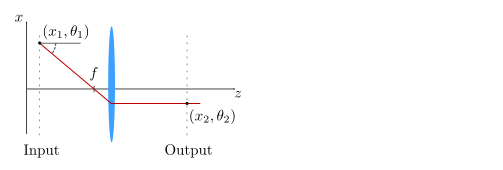
\includegraphics[width=\textwidth]{RTM.pdf}	
\caption{Sketch of a light ray moving through an optical system. It first hits a mirror and is reflected, next it passes through a lens and is refracted. \label{fig:RTMA}}
\end{figure}

In the figure $z$ is the optical axis and $x$ is axis orthogonal to the optical axis. We define two planes transversal to the optical axis, we name the first the \emph{input}-plane and the second the \emph{output}-plane. Note that we can classify all aspects of the ray as it crosses either planes by two parameters: the distance from the optical axis $x_1$ and the angle it has to the optical axis $\theta_1$.

When passing through the system, the ray has been changed from $(x_1, \theta_1)$ to $(x_2, \theta_2)$. These two vectors can be connected by the use of a general matrix $M$, so we have
$$\begin{pmatrix}
	x_2 \\ \theta_2
\end{pmatrix} = 
\begin{pmatrix}
	A & B \\ C & D
\end{pmatrix}
\begin{pmatrix}
	x_1 \\ \theta_1
\end{pmatrix}.
$$
The matrix $M$ is usually referred to as the \emph{transfer matrix}, which explains the name of the method. As the components of the matrix are completely general we have just named them $A$, $B$, $C$ and $D$---this is actually quite common, and another popular name for tranfer matrix analysis (TMA) is actually just the ABCD-method.

For any optical system, there is necessarily a transfer matrix that will connect any input and output planes. This lets us see any optical system as a black box. It doesn't necesarily matter how the system is set up, as long as we know the transfer matrix for the system, we can calculate the output of any input ray. If we connect two such black-box optical systems together the total transfer matrix is simply the matrix-matrix product $M=M_1M_2$.

So we see we have a very general method that is also conceptually simple. However, we still don't really know how to find the transfer matrices in the first place. For most simple optical components such as straight and curved mirrors and lenses the matrices can be found analytically from Maxwell's equation. For other components, the transfer matrix can be found experimentally. When setting up our system, we simply multiply the sequence of all the components to find the total transfer matrix for the system.

\subsubsection{The Beam Parameter}

So we have seen that the ray tranfser matrix analysis method is both simple and usefull. However, it is based on the ray assumption of light. In this project we are looking at beams, not rays. Luckily, there is a simple way to extend the transfer matrix analysis formalism to beam optics.

We do this by introducing the complex \emph{beam parameter}
$$\frac{1}{q} = \frac{1}{R} - \frac{i\lambda}{\pi n w^2},$$
where $R$ is the radius of curvature and $w$ is the beam spot size, i.e., the width of the beam. We will explain these quantities in more detail in the next section. We also need the wavelength of the beam $\lambda$ and the refractive index $n$. 

With the introduction of this beam parameter, we can define a \emph{beam}-vector, which is simply $(q,1)$. With the introduction of this beam-vector, we can use the transfer matrix analysis also for beams. When multiplying a beam-vector with a given transfer matrix, the second component of the beam-vector might change, we therefore introduce a \emph{renormalization-constant}, $k$, which holds the second component of the beam-vector at unity.

Note that with the introduction of the beam parameter, we no longer keep track of the angle the beam has to the optical axis, we now instead look only at the width of the beam and the radius of curvature. 

\subsection{Gaussian Beams}

A gaussian beam is a beam where the intensity profile of the beam transversal to the propagation-direction of the beam follows a gaussian distribution, such a distribution is shown in figure \ref{fig:gauss_dist}.

As mentioned earlier, in beam optics we usually work under the assumption of gaussian beams, and a lot of the results will not be valid for non-gaussian beams. The TMA method for beams also uses this assumption.

\begin{figure}[htpb]
\centering
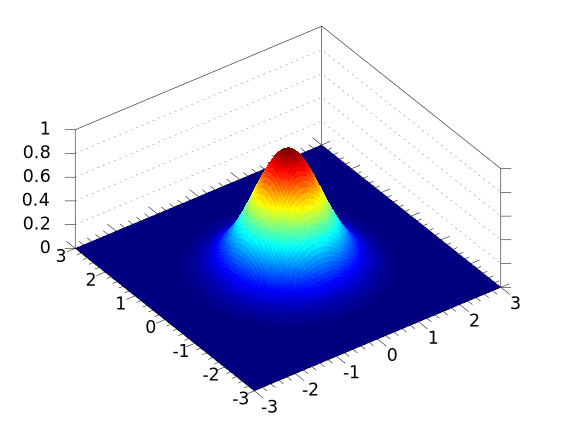
\includegraphics[width=0.7\textwidth]{Gaussian_2d}	
\caption{Sketch of a 2D Gaussian distribution with amplitude and standard deviation equal to unity. \label{fig:gauss_dist}.}
\end{figure}

\clearpage

An important fact of beam optics, is that a beam that is \emph{not} gaussian, will usually become more gaussian as it undergoes diffraction as it passes through optical devices. If we then start of with a gaussian beam, the profile of the beam won't be changed by introducing more lenses or removing lenses. But for a non-gaussian beam, introducing a lens might significantly change the profile of the beam.

The fact that a beam is gaussian also means we can define the width of the beam. We let the width be defined as two times the standard deviation of the beam, meaning it is equal to the distance we have to move away from the center of the beam to hit the point where the intensity has fallen to $1/e^2$ of the peak value.



\subsubsection{The Beam Waist}
We can now use TMA to calculate how a Gaussian beam travelling undisturbed through a vacuum will develop. An important observation when this is done is that a beam will never have a constant width, but will instead either become more narrow or wider as it goes due to diffraction. Which of these it does is classified by the \emph{radius of curvature}, $R$, which was one of the parameters that went into defining the beam parameter.

A positive radius of curvature means that the beam will become wider over time, while a negative radius of curvature means the beam will narrow. Let us look closer at what happens when a beam with a negative radius of curvature narrows, the development of such a beam is shown in figure \ref{fig:gaussian_beam}.

We see that the beam narrows down to a minimum, and then starts expanding again. The point where the beam is at its narrowest is often referred to as the \emph{waist} of the beam. We denote the width of the beam at the waist as $w_0$. The distance from the waist to the point where the area of the beam has doubled is reffered to as the \emph{Rayleigh range}, $Z_{\rm R}$. The beam is symmetric around its waist, meaning we can move $Z_R$ to either direction from the waist, and the width of the beam will be $\sqrt{2}w_0$. If we move much further than the Rayleigh range away from the waist, the width of the beam will increase linearily. The angle formed between the optical axis and the beam far from the waist is called the divergence of the beam, which we will denote $\theta$.

\begin{figure}[htpb]
\centering
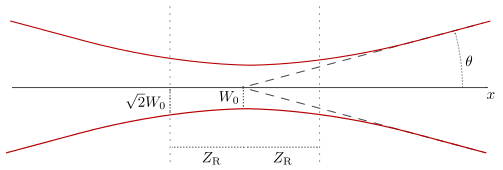
\includegraphics[width=\textwidth]{beam.pdf}	
\caption{Sketch of how a Gaussian beam changes when close to its minimum width. \label{fig:gaussian_beam}}
\end{figure}

An important fact here, is that the beam is symmetric about its waist. This means if a beam is focused into a waist that is close, it will also expand quickly again after passing through its waist. From TMA we can show that the divergence of a gaussian beam is given by
$$\theta = \frac{\lambda}{\pi w_0}.$$
So we see that the width of the waist is inversely proportional to the divergence. This results mean two important things for beams. If we want to focus a beam down to the smallest possible point, we want a small waist, and so the divergence must be as big as possible. But if we want a beam with a small divergence, we need to have a wide a beam as possible.

\subsubsection{Beam Quality}

As explained so far, we work under the assumption of Gaussian beams, and such beams are practical to work with, as their profile is maintained even when passing through many optical devices. However, we will now see that a gaussian beam also has an important quality when using a lasers in industry.

First we define the \emph{beam parameter product}, which is the product of the width of the waist and the divergence of a beam, so 
$$\mbox{BPP} = w_0\cdot\theta.$$
For a Gaussian beam, this will be a very simple quantity to compute
$$\mbox{BPP}_{\rm Gaussian} = w_0\cdot\theta = \frac{\lambda}{\pi}.$$
While for any other beam, we can find the BPP experimentally by simply measuring $w_0$ and $\theta$. It can be shown that any non-gaussian beam will have a bigger BPP than the Gaussian beam, which means it effectively will have a bigger waist for the same divergence.

Due to the fact that 
$$\mbox{BPP}_{\rm Gaussian} \leq \mbox{BPP},$$
we can define a meaningful measure of \emph{how gaussian} a general beam is from the quantity
$$M^2 = \frac{\mbox{BPP}}{\mbox{BPP}_{\mbox {Gaussian}}}.$$
Any laser-beam will have $M^2 \geq 1$, where the closer to unity the $M^2$ quantity is, the closer the beam is to a gaussian one.

The quantity $M^2$ is often known as the \emph{beam quality}. If we focus a real laser beam down to its waist, the waist will by $M^2$ wider than the theoretical possible minimum value. This means that when one builds a laser, there is usually a clear goal to keep the beam quality as close to unity as possible so that the beam is as gaussian as possible.

\subsection{Optical devices}

\subsubsection{Lenses}

A lens is a transmissive optical device, meaning light passes through it. The light that passes through a lens is changed due to diffraction. Many different lenses can be built, but we will limit our discussion to simple biconcave and biconvex lenses.

\begin{figure}[htpb]
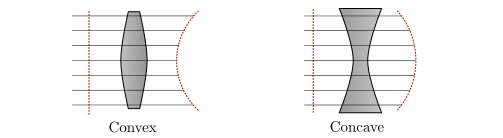
\includegraphics[width=\textwidth]{lenses.pdf}	
\caption{Sketch of the optical path of the different parts of a beam that passes through an abstract lens. \label{fig:lenses}}
\end{figure}

An abstract, idealized lens only changes the radius of curvature $R$ of the beam that passes through it. To understand how the curvature is changed, it is helpful to think of the optical path of different parts of the beam. Figure \ref{fig:lenses} shows schematically a beam pasing through a biconvex and a biconcave lens. As a lens is generally made of a material with a higher index of refraction than air, light passes through the lens slower than in the air. This means that the parts of the beam that passes through the thinnest parts of the lens can move further away from the lens than the the parts of the beam that has to pass through the thickest part of the lens. 

If we then draw a virtual line through the parts of the beam with the same phase after it has passed through the lens, we see how the curvature has been affected. Assuming the beam had a completely planar curvature before the lens, a convex lens will change the curvature to a positive one, while the concave lens will make it negative. More specifically, the curvature will be equal to focal length of the lens.

As should be apparent, the situtation shown in figure \ref{fig:lenses} does not require the beam to pass from left-to-right. The lenses are symmetrical and so the light could just as easily move from right-to-left. This means that a beam which has a curvature equal to the focal length of a lens will be turned into a planar wave by passing through that lens. We use this fact when we construct a beam expander.

\subsubsection{Beam Expanders and Narrowers} \label{sec:beam_expander}

The goal of a beam expander is to increase the width of a beam without changing it's radius of curvature. Such a device can be made in different ways, but let us look at a simple setup using two biconvex lenses. A sketch of a possible setup is shown in figure \ref{fig:beam_expander}

\begin{figure}[htpb]
\centering
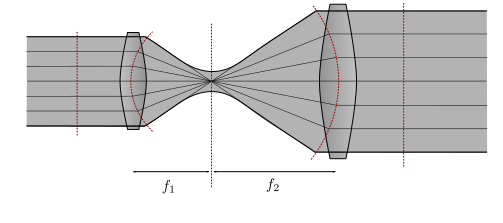
\includegraphics[width=\textwidth]{beam_expander.pdf}	
\caption{Sketch of a beam passing through a beam expander made from two biconvex lenses. \label{fig:beam_expander}}
\end{figure}

If we assume a planar beam hits a convex lens the curvature will become positive, this is explained in the previous section. Due to the curvature of the beam, it will narrow as it continues after the lens, hitting it's minimum width at the focal length of the lens. After passing the minimum it will expand again, meaning the curvature has become negative. If we place another convex lens at the right distance the beam can again become planar by passing through it. For this to happen, the lens has to be placed so that the distance from the waist to the lens is preciesly equal to it's focal length. The net result is that a planar wave has been expanded without any alteration in the curvature. 

Just as in the previous example, there is no preference for the beam to pass from left-to-right in the sketch, meaning we can just as easily create a \emph{beam narrower} from two biconvex lenses. The difference between the expander and narrower is simply which lens has the biggest focal length. If the first lens has a smaller focal length, i.e., $f_1 < f_2$ the beam is expanded and vice versa. In fact, for our example with plane waves, it can be shown that the width is increased or decreased by a factor of $M = f_2/f_1$, which confirms our statement. 

\section{Experiments}

\subsection{Experiment 1: Finding the Radius of Curvature of a beam}

The first experiment we conducted in the lab had the goal of finding the radius of curvature of a laser beam. We have a beam profiler that can measure the width of the beam, but we have no way to measure the radius of curvature directly. Instead we measure the width at various points along the beam. These measurements lets us use a numerical TMA calculation and a least squares parameter fitting to find the radius of curvature that best fits with our measurements. 

\subsubsection{Method}

This experiment was conducted using a Helium-Neon (HeNe) laser as our beam source. The laser itself generated a beam of a constant, non-adjustable, intensity. The  beam was therefore passed through an optical setup that let us adjust the intensity of the resulting beam. A picture of the optical setup is shown in figure \ref{fig:setup_photo} and a sketch of the setup is shown in figure \ref{fig:setup_sketch}. The reason this setup is used is that it gives us the ability to adjust the intensity of the beam by rotating the half-wave plate (HWP). The HWP rotates the plane of polarization of the beam, and so different amounts of the beam are transmitted through the second polarizing beam-splitter (PBS).

A beam profiler was put into the beam's path to measure the width of the beam at various distances. First the beam was left unhindered and simply measured at various distances. Then a new set of measurements were taken of the beam after a lens of focal length $f_1=100$ mm was put into the path of the beam.

The reason the beam intensity needs to be adjusted is that as the beam expands, the intensity decreases. If the intensity is to low, the beam profiler can't find a good width of the beam, if the intensity is too high, the signal is clipped in the beam profiler and we have the same problem. The intensity of the beam is therefore adjusted every time the beam profiler is moved.

\begin{figure}[h!t]
\centering
\includegraphics[width=\textwidth, angle=180]{oppsett_photo}	
\caption{Photo of the optical setup. After being reflected in the mirror on the right-hand side on the picture, the beam travels a measured distance before hitting a beam profiler which measures the transversal intensity of the beam. \label{fig:setup_photo}}
\end{figure}

\begin{figure}[t!]
\centering
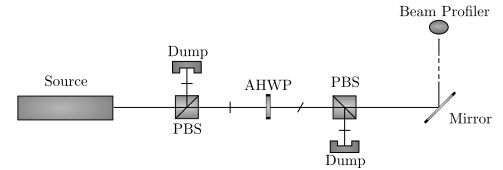
\includegraphics[width=\textwidth]{oppsett1}	
\caption{Sketch of the optical setup. The laser beam passes from the source through a polarizing beam splitter (PBS). Roughly half of the light is then reflected and passed to a dump, the transmitted light will be linearily polarized along a given axis. Next the linearily polarized light passes through an adjustable half wave plate (AHWP), which rotates the polarization-plane. Next, the beam passes through another PBS and the reflection is again captured by a dump. The amount of light that is now reflected depends on how much the polarization has been rotated by the AHWP. The transmitted part of the beam is reflected by a mirror and travels a measured distance before hitting a beam profiler, which measures the transversal intensity of the beam. \label{fig:setup_sketch}}
\end{figure}

\begin{figure}[ht!]
\centering
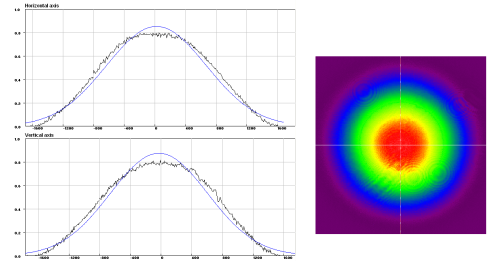
\includegraphics[width=\textwidth]{beampro.pdf}	
\caption{Output from the beam profiler at the computer. At the top, the intensity of the beam transversal to the propagation is shown. Below the intensity along the horizontal and vertical axises are shown. A gaussian fit is plotted over the measured intensity and the width of the fit is printed out. For the plots the $y$-axis shows the elative intensity and the $x$-axis is the distance from the origin in $\mu$m. \label{fig:beam_pro}}
\end{figure}

\clearpage

Figure \ref{fig:beam_pro} shows the output of the beam profiler. Note that what is measured is the width of a gaussian fit to the measured intensity of the beam. As the beam is not perfectly gaussian, this is a source of error that very well might be systematic.

\subsubsection{Results}

The results of the experiment is shown in figures \ref{fig:e1r1} and \ref{fig:e1r2}, both on the next page. In both figures the measured widths and the best TMA fit is shown.

\subsubsection{Discussion}

In figure \ref{fig:e1r1} we see the measurements of the unhindered beam. We see that the beam starts out with a low divergence but after about $500$ mm it quickly starts expanding, tripling in width over the next meters. The best TMA fit to the complete data set, if we let the starting width of the calculation be equal to the first measurement, was found to be $R_0\approx 3000$ mm. The fit looks quite good, but we see there is a systematic error both in the first few points, as the fit undershoots slightly in the beginning and overshoots slightly in the end. This effectively means the divergence of the measurements is smaller than the TMA fit.

In figure \ref{fig:e1r2} the fit looks much better in general. The estimated radius of curvature is equal to the focal length of the lens, which fits the theory very well. From the measurements we can estimate the beam quality of the beam. As we have both a clear waist and measurements far outside the Rayleigh range we can read of both the width of the waist, $w_0$ and the divergence of the beam $\theta$. This lets us estimate the BPP of the beam and thusly the beam quality $M^2$. It turns out the $M^2$-value turns out to be 0.999 from our measurements, which as explained earlier, is not theoretically possible. In fact, from figure \ref{fig:e1r2} you can see the theoretical TMA fit is actually the worst for the measurements around the waist, and this is probably due to it being physically impossible---remember that the TMA fit follows the path of a Gaussian beam, which cannot reach a slimmer waist than it already does for the given divergence.

The exact explanation for both the too low divergence for the unhindered beam and the error in the beam quality is probably caused by a combination of many different errors, but one quite large source of error is seen from figur \ref{fig:beam_pro}, the output of the beam profiler. As we read of the width of the fit, and not the beam itself, from the picture we can see a clear systematic error of measuring a too slim width. A narrower beam leads to a both a higher divergence and a lower BPP, and thus a better $M^2$-value. HeNe-lasers are known for having excellent beam quality, meaning the true value of $M^2$ for the beam is probably very close to unity already, so even a small systematic error can push the $M^2$-value below unity.

\begin{figure}[p]
\centering
\includegraphics[width=\textwidth]{experiment_1}	
\caption{Measured width of the beam passing unhindered through air and the best TMA fit superimposed. The radius of curvature was estimated to be approximately $R_0 \approx -3000$ mm at $l=0$. \label{fig:e1r1}}
\end{figure}

\begin{figure}[p]
\centering
\includegraphics[width=\textwidth]{experiment_1_wlens}	
\caption{Measured width of the beam after passing through a biconvex lens positioned at $l=0$ with focal length 100 mm. The best TMA fit is superimposed. The radius of curvature was estimated to be approximately $R_0 \approx -100$ mm at position at $l=0$. \label{fig:e1r2}}
\end{figure}

\clearpage

\subsection{Experiment 2: Measuring the effects of a Beam Expander}

In our second experimental set up, we have the goal of making a beam expander from two biconvex lenses, and the study how the beam is affected when passing through it. We also study the effects of small adjustment to the distance between the two lenses which compromise the beam expander.

\subsubsection{Method}

As before, we have a biconvex lens with a focal length $f_1 = 100$ mm, we position this at $200$ mm, we introduce another biconvex lens at $500$ mm, this with a focal length of $f_2=200$ mm. As the first lens has a smaller focal length than the second, and the distance between the lenses is equal the the sum of the focal lengths, the two lenses make a beam expander, as explained in section \ref{sec:beam_expander}. Three sets of measurements are done, where the distance between the lenses is varied a few mm between every set.

\begin{figure}[ht]
\centering
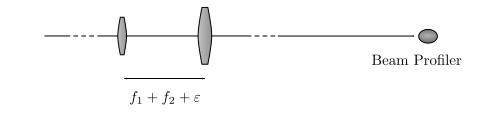
\includegraphics[width=\textwidth]{oppsett2}	
\caption{The beam expander used in experiment 2. The distance between the lenses is equal to the focal lengths, pluss a small offset $\eps$. \label{fig:e2}}
\end{figure}

\subsubsection{Results}

The results are shown in figures \ref{fig:e2r1}, \ref{fig:e2r2}, \ref{fig:e2r3}. Here, the first data set had a slight negative offset in the distance of 3 mm, while the third data set had a positive offset of 3 mm, the middle data set had no offset.

\subsubsection{Discussion}

One should note that the results up untill the second lens is the same for all three data sets, this should of course be the case, as the only thing that is changed between the measurements is that the second lens is moved. The measurements before the second lens are the same measurements as in the second part of the first experiment. Just as in that experiment, we see that the measured waist is to slim, and the TMA fit does not manage to reproduce it.

However, the interesting part of these plots is what happens after the second lens, where we see very different behaviors even though the adjustments to the distance between the lenses was quite small. In all three cases, the beam goes from roughly 400 $\mu$m to 800 $\mu$m in width, meaning we have a magnification factor of $M=2$. This fits with the theory we have presented earlier. However, the radius of curvature is altered by the adjustment in the offset. In the first two data sets, we see the divergence is very small and the beam is near constant in width. For the last data set, the divergence is negative, and the beam is narrowing over a long distance after the second lens.

For all three data sets, the fit is a lot worse in this experiment than it was in the previous experiment. The reason for this is probably a several factors, but one of them being that the TMA analysis assumes thin, idealized lenses. While we in the experiment have thick lenses, with non-exact focal lengths and so on.

\begin{figure}[h!t]
\centering
\includegraphics[width=0.9\textwidth]{beam_expander_dataset_0.pdf}	
\caption{Measurements and best overall TMA fit when the distance between the lenses has a slight negative offset, $\epsilon = -3$ mm. \label{fig:e2r1}}
\end{figure}

\begin{figure}[ht]
\centering
\includegraphics[width=0.9\textwidth]{beam_expander_dataset_1.pdf}	
\caption{Measurements and best overall TMA fit when the distance has no offset. \label{fig:e2r2}}
\end{figure}

\begin{figure}[ht]
\centering
\includegraphics[width=0.9\textwidth]{beam_expander_dataset_2.pdf}	
\caption{Measurements and best overall TMA fit when the distance has a slight positive offset, $\epsilon=3$ mm. \label{fig:e2r3}}
\end{figure}

\clearpage

\subsection{Experiment 3: Long-distance measurements of a laser beam}

For the final experiment, we want to perform measurements of a laser beam sent over a long distance. From theory we know that the divergence of the beam will be smaller if we let it start big, and it is this fact that we are most interested in testing out in practice.

\subsubsection{Method}

For the final outdoor experiment a green laser pointer with wavelength $\lambda = 532$ nm is used as the source. The beam is sent a distance of roughly 710 m before hitting a piece of cardboard. See figure \ref{fig:map} for a map of the surrounding area. A telescope is then used as a beam expander to expand the beam at the origin.
The telescope uses an ocular with a focal length of $f_1 = 14$ mm and an objective with a focal length of $f_2 = 810$ mm. After being expanded the beam is again observed at the same distance from the source. By focusing the telescope, i.e., adjusting the distance between the two lenses, we can move the waist of the beam. We do this until we make the beam spot size as small as we can at the measurement end---this effectively means adjusting the beam expander adjustment so that the waist is placed precisely at the measurement position.

In addition to this, we measure the beam of the laser pen in the lab to get a measure of the starting width and radius of curvature of the beam, as well as a feel for how gaussian the beam actually is.

\subsubsection{Results}

In figure \ref{fig:lp_profile} the beam profile of the laser pen is shown after the beam has passed roughly 200 mm unhindered through air. In figure \ref{fig:e3r1} measurements of the laser beam in the lab and the best TMA fit is shown. Figure \ref{fig:e3r2} shows the resulting beam spot at the measurement end when the laser beam is sent unaltered from the source on the left, and when the beam is expanded by the telescope and focused on the right. In figure \ref{fig:e3r3} we show the result of a TMA analysis, where we use the the measurements on the laser pointer from the lab to calculate the beam spot size at the measurement point. The distance between the two lenses in the telescope is adjusted to move the waist as close to the measurement point as possible

\begin{figure}[ht]
\centering
\includegraphics[width=0.7\textwidth]{map.jpg}  
\caption{Map showing the path of the beam, the distance from the source to the point of measurement is estimated to be roughly 710 m.\label{fig:map}}
\end{figure}

\begin{figure}[ht]
\centering
\includegraphics[width=\textwidth]{laserpenn_vh}  
\caption{Measurements of the beam from the laser pen and best TMA fit.  \label{fig:e3r1}}
\end{figure}

\begin{figure}[ht]
\centering
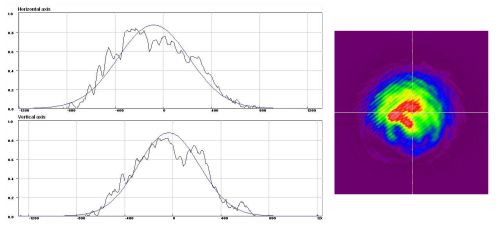
\includegraphics[width=\textwidth]{laserpen}  
\caption{Output from the beam profiler for the laser pointer.  \label{fig:lp_profile}}
\end{figure}


\begin{figure}[p]
\centering
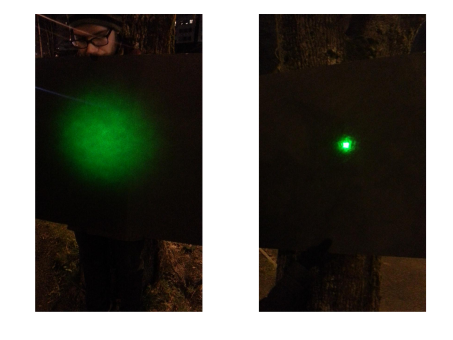
\includegraphics[width=\textwidth]{experiment3}  
\caption{Final beam spot size of the unaltered laser beam on the left, and of the expanded beam on the right. The cardboard plate shown has dimensions 70$\times$100 cm, which lets us estimate the spot size. \label{fig:e3r2}}
\end{figure}

\begin{figure}[p]
\centering
\includegraphics[width=\textwidth]{e3p3}  
\caption{TMA results of the beam travelling a long distance after passing through the telescope when the distance between the lenses is set to $f_1+f_2+\eps$ and the offset $\eps$ is adjusted. The vertical line shows the measurement point where we want the waist to hit. \label{fig:e3r3}}
\end{figure}

\clearpage

\subsubsection{Discussion}

From the measurements shown in figure \ref{fig:e3r1}, we can see that the beam from the laser pen starts out with with a beam spot size of roughly 550 $\mu$m and a very large radius of curvature. We see that the fit is only good for the first few measurements, but it starts expanding much faster than the actually measurements. After looking at the beam profile in figure \ref{fig:lp_profile}, this isn't terribly surprising, as the beam is very far from being a neat gaussian profile, and so the TMA results will naturally be poor. The radius of curvature found from a least squares parameter fitting was $2.7\cdot10^{11}$, meaning the beam starts out with a nearly completely flat curvature.

If we put the start-width of the beam and the huge radius of curvature into the TMA-method and let the beam pass unhindered $710$ meters through air, we get a final beam spot size of about 109 mm. We can estimate the actual beam spot size from figure \ref{fig:e3r2}, we know the cardboard plate is 70 cm in height in the picture, from that we measure that area of the plate that is illuminated is roughly 48 cm in diameter. Now, we can't read of the intensity of the beam of the picture in any meaningful way, as the camera does not represent the intensity in a linear way. Also, we don't know where the cutoff of the camera is, i.e., the lowest intensity the camera can pick up. However, since we can see a spot of roughly 48 cm in diameter, the radius is roughly 24 cm. Remembering that the beam width is defined as the radius, and not the diameter, we see there is actually a decent correspondance between the the theoretical and the experimental result.

Next, we turn to the measurement with the telescope beam expander. We put the two lenses into the TMA calculation, with a distance of $f_1+f_2+\eps$ between them, where $f_1=14$ mm and $f_2=810$ mm are the focal lengths of the two lenses, we also include a small offset $\eps$, just like in experiment 2. From figure \ref{fig:e3r3} we see the effects of altering the the offset ever so slightly. Even though the distance between the lenses is already $824$ mm without an offset, changing the distance by even a half millimeter changes the results drastically! In each case, the beam has the same starting width of roughly 65 mm, but the beams with a positive offset narrow significantly as they propagate. Also note that for the beam without an offset, the beam is very near constant. This confirms our theory that a beam that starts out wide has a low divergence. 

Using parameter fitting on the offset $\eps$ we can find the exact offset needed to move the waist to the measurement point. This is effectively the same as what we did when we focused the telescope untill the beam spot size was at a minimum. When we do this we get a theoretical beam spot size of 1.88 mm at the measurement point. From figure \ref{fig:e3r2} we estimate that the diameter of the visible spot is about 4 cm. This means that the observed spot is quite a lot wider than the theoretical prediction. This is not that strange, as actually hitting the exact waist in practice is really hard due to the beams sensitivity in the offset. The TMA is also the prediciton for a gaussian beam, which as described in the beginning of this report has the smallest possible waist of any beam. We have seen that the laser pointer does not produce a very gaussian beam, and so we expect the waist to be quite a bit wider than the theoretical prediction.



\clearpage

\section{Estimations of beams used in Moon-measurements}

The National Aeronautics and Space Administration (NASA) uses laser beams to measure the distance to the moon. In several of the Apollo missons, reflector plates have been left on the surface of the moon. These have the property that they reflect the light that hits them back in the same direction. This lets the part of laser beam from earth that hits the reflector plate be passed back down to the origin of the laser. By measuring the time from a pulse is sent out, to a reflection is observed, one can very accurately measure the distance to the moon. Figure \ref{fig:reflector} shows the reflector plate left by the Apollo 11 mission.

\begin{figure}[hptb]
\centering
\includegraphics[width=\textwidth]{Apollo_11_Lunar_Laser_Ranging_Experiment}  
\caption{The reflector plate left behind by the Apollo 11 mission. The picture is public domain. \label{fig:reflector}}
\end{figure}

From the picture, we see that this reflector plate is quite small, on the magnitude of $1\times1$ m. As we have seen in our experiments, keeping a beam at constant width is almost impossible, so how can it be that they manage to use a plate of such a small size to reflect a laser beam that has travelled such a long distance? Let us make some quick estimations to see how this can be done.

We are only interessted to check the feasability of the method, so we don't really need exact measurements, as long as they are of the correct order of magnitude. Let us assume that the reflector plate has an area of 1 m$^2$. Let us say they use a telescope of diameter 3.5 m to both expand the beam, and catch the reflected light from the moon. We then set the starting width of the beam to be about 1 m. The distance from the earth to the moon is roughly 384400 km. We then choose a very large radius of curvature to have the beam have the smallest divergence possible. It is true that the we would like to place the waist of the beam the closest to the moon as possible, but as the distance to the moon is so much larger than the diameter of the beam in the first place, there is nothing to be gained from this. When the light hits the reflector plate, we let the plate act as a new beam source. Let us just assume that the plate is round and reflects a perfect gaussian beam, which is definitly not the case, but let us assume for the sake of argument. The result of the TMA of the given estimates is shown in figure \ref{fig:moonTMA}

\begin{figure}[htbp]
\centering
\includegraphics[width=0.6\textwidth]{moon_beams}  
\caption{Result of a TMA analysis of the beam traveling from Earth to the moon and back. \label{fig:moonTMA}}
\end{figure}

We see that beam spot size grows from about 1 m to about 65 m both ways. This is actually an impressively small growth over the vast distance the beam has travelled. As the area of the beam grows proportional to $w^2$, we see there is a lot of energy loss, as only a small fraction of the beam is reflected from the moon, and then only a small fraction of the reflected beam is absorbed back at the telescope. From our results we expect the return signal to be roughly $10^{-7}$--$10^{-8}$ times smaller than the outgoing signal, and that is only accounting for the expansions of the laser beams, one also expects some energy loss from scatterings in the atmosphere. It is quite impressive that this is enough to measure the distance from the earth to the moon.



\clearpage

\section{Summary}

We started this report by giving a quick introduction to ray optics and the ray transfer matrix analysis method for calculating the path of rays. We saw that ray optics is a simplified subset of optics based on a few key assumptions, namely the paraxial/small-angle approximation and that the wavelength of the light in question is small. Analogously beam optics is a simplified subset of optics based also on the paraxial approximation and the assumption that all beams have a gaussian intensity profile. Under these assumptions we saw the path of a laser beam can be predicted using the transfer matrix analysis. 

From the TMA we saw that a laser beam will not have a constant width, but will either get wider or slimmer as it propagates due to diffraction. When focused down to a spot, a laser beam cannot get arbitrarily narrow, but will instead hit a waist before expanding again. The angle of a divergence of a beam is a key quantity when describing a laser beam, as it tells us how fast a beam will spread out. We have seen that for a gaussian beam this angle is inversely proportional to the waist size, meaning a beam that starts out wide will be much better at staying roughly the same width, while a beam that is relatively thin must spread out. We have also seen that for a given angle of diffraction, the waist of a gaussian beam will be smaller than that of any other beam profile, and this fact is used to classify the beam quality of a general laser beam.

Through experiments where we measured the width of a laser beam, we have estimated the radius of curvature of the wavefront of the beam by using a least-squares parameter fitting of a TMA-analysis that tries to reproduce the measurements. We saw that this approach worked well for a HeNe-laser where there is a high beam quality. However, we also noticed that due to systematic measurement-errors, our results where inconsistent with theory, as the measurements had a beam quality of less than unity, which should not be physically possible.

Through experiment, we also studied beam expanders made from two biconvex lenses. We saw how even small adjustments in the distance between the lenses had a huge impact of the radius of curvature of the beam after passing through the expander, while the magnification of the beam was unaltered from the offset in distance.

Finally we measured the width of the beam from a laser pointer after nearly a kilometer. Even though the beam from a laser pointer starts out narrow, we found that it quickly grew in width. To be able to have a thin beam at the measurement point we had to create a beam expander from a telescope. When expanding the width of the beam more than 50-fold the beam was so wide that it had almost no divergence at all when passing a kilometer. However, the real pay-off came by adjusting the distance between the lensen in the beam-expander, as this let us give the beam a negative radius of curvature, making it narrow as it propagated toward our target. By adjusting the distance exactly right, we could place the waist of the beam on our target, focusing the laser down to a very small spot.

We ended by looking at a real-world use of our result, measurements of the earth-moon distance. To get a good reflected signal from the moon, one requires a small beam divergence, which means the beam has to start wide. This result may be counter-intutive, but as we have seen, it is supported by both theory and experiment.








\clearpage


\section{Sources} 

[1] McGraw-Hill, 1993. \emph{Encyclopedia of Science and Technology, 5th ed.}.

[2] Vistnes, Arnt-Inge, 2013. \emph{Svingninger og bølger}. Digitale utgivelser ved UiO.

[3] \url{http://en.wikipedia.org/wiki/Ray_transfer_matrix_analysis}

[4] \url{http://en.wikipedia.org/wiki/M_squared}, november 2014

[5] \url{http://en.wikipedia.org/wiki/Diffraction}, november 2014

[6] \url{http://en.wikipedia.org/wiki/Gaussian_beam}, november 2014

[7] \url{http://en.wikipedia.org/wiki/Beam_parameter_product}, november 2014

[8] \url{http://en.wikipedia.org/wiki/Lunar_Laser_Ranging_experiment}, november 2014

[9] \url{http://alomar.rocketrange.no/sodium.html}, november 2014











\end{document}